\chapter{Resultados}
\label{chap:resultados}

% TODO Inlcuir datos de las máquinas

\section{TFHE}

\subsection{Tiempos de ejecución}

Al ser una ejecución "especulativa", la optimización de las funciones está muy limitada (se tiene que operar con todos los bits, gestionando el flujo de los datos eligiendo los valores con los que se opera mediante la puerta \verb|MUX|). Sin embargo, siempre que el circuito lógico sea cerrado para un número concreto de bits (de forma similar a un circuito físico), pueden utilizarse métodos formales y algebraicos para aumentar su eficiencia.

Por otro lado, crear algoritmos que sean versátiles con respecto al número de bits hace que estos circuitos lógicos tengan que hacer operaciones redundantes, o introducir demasiada complejidad ciclomática para estar preparado para cualquier tamaño de palabra.

\subsubsection{Operaciones aritméticas}

Según la documentación de TFHE, cada puerta lógica tarda 13ms en ejecutarse, y las puertas MUX tardan 26ms. Sabiendo que sólo el $ 13\% $ de las puertas lógicas en nuestro código son puertas MUX podemos establecer un tiempo por puerta de unos 15ms para calcular el tiempo teórico que deberían tardar nuestras operaciones en función del número de puertas lógicas que emplean. En la tabla \ref{table:time_by_gates} podemos ver los resultados del cálculo.

\begin{table}[]
    \centering
    \begin{tabular}{r | cc}
        operación       & puertas logicas       & tiempo estimado \\
        \hline \hline
        compare\_bit     & 2     & 0,04 \\
        equal   & 128   & 2,56 \\
        is\_negative     & 1     & 0,02 \\
        minimum/maximum & 388   & 7,76 \\
        add\_bit & 5     & 0,1 \\
        sum     & 320   & 6,4 \\
        negativo        & 192   & 3,84 \\
        resta   & 512   & 10,24 \\
        multiply        & 46826 & 936,52 \\
        mayor\_igual     & 128   & 2,56 \\
        shiftl/shiftr   & 771   & 15,42 \\
        u\_shiftl/u\_shiftr       & 129   & 2,58 \\
        divide  & 85776 & 1715,52 \\
    \end{tabular}
    \caption{Tiempo estimado de ejecución}
    \label{table:time_by_gates}
\end{table}

Hemos medido los tiempos de ejecución de las distintas operaciones aritméticas con varios tamaños de palabra (de 4, 8, 16, 32 y 64 bits). En la figura \ref{fig:crec_func} podemos observar como prácticamente todas tienen un crecimiento lineal con mayor o menor pendiente: hay algunas que son casi gratuitas, como las operaciones \verb|shift|; y hay otras como la resta, que crecen un poco más rápido (porque están compuestas por varias operaciones crecientes) pero sin perder su comportamiento lineal.

\begin{figure}[h]
    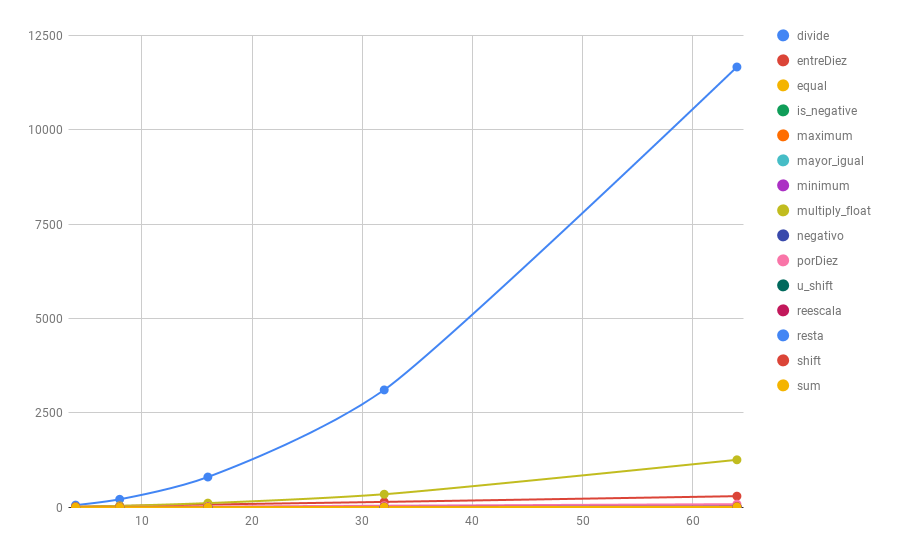
\includegraphics[width=\textwidth]{crec_func}
    \caption{Tiempo de ejecución por número de bits}
    \label{fig:crec_func}
\end{figure}

Sin embargo hay dos operaciones que crecen de una forma más preocupante: la multiplicación y la división. En ambas funciones se juntan tres factores:

\begin{enumerate}
    \item Requiere el uso de un gran número de funciones adicionales: sumas, restas, comparaciones, etc; haciendo que crezca el número de puertas lógicas.
    \item Debido a su complejidad, tiene varios bucles anidados cuyas iteraciones están relacionadas con el número de bits.
    \item Abordamos las operaciones trabajando con el doble de bits de la entrada. Es decir, un número de 64 bits se opera como si tuviese 128 para evitar desbordamientos.
\end{enumerate}

En la tabla \ref{table:ops_real_time} vemos cuáles son estos tiempos con números de 64 bits.

\begin{table}[]
    \centering
    \begin{tabular}{cc}
        Operación       & Tiempo (s) \\
        \hline \hline
        compare\_bit     & 0 \\
        is\_negative     & 0 \\
        u\_shift       & 0 \\
        add\_bit & 0 \\
        equal   & 3 \\
        mayor\_igual     & 4 \\
        min / max & 14 \\
        sum     & 8 \\
        negativo        & 8 \\
        resta   & 16 \\
        shift   & 19 \\
        multiply        & 1257 \\
        divide  & 11662
    \end{tabular}
    \caption{Tiempo real de ejecución}
    \label{table:ops_real_time}
\end{table}

En la figura \ref{fig:crec_div_mult} se puede ver cómo el crecimiento de cada valor con respecto al anterior  ($f(2^x)/f(2^{x-1})$ con $x$ número de bits) de ambas funciones corresponde con un crecimiento potencial con respecto al número de bits.

\begin{figure}[h]
    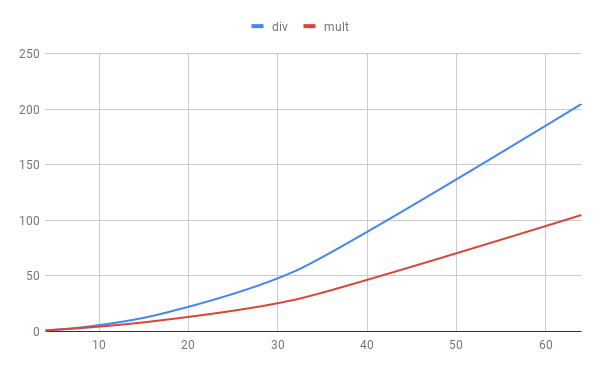
\includegraphics[width=\textwidth]{crec_div_mult}
    \caption{Crecimiento: división y multiplicación}
    \label{fig:crec_div_mult}
\end{figure}
% ---

Por último, calcularemos el tiempo teórico que tardarían en realizarse las operaciones de la curva de regresión (sumando los tiempos de sus sumas, multiplicaciones, divisiones...) y lo compararemos con el tiempo que han tardado realmente.

En la tabla \ref{table:sub_ops_r2} analizamos las operaciones contenidas en cada uno de los cálculos (ver anexo \ref{appendix:regresion_cuadratica}) y el tiempo estimado que tardarían en función de los tiempos mostrados en la tabla \ref{table:ops_real_time} .

\begin{table}[]
    \centering
    \begin{tabular}{r | c c c c}
        Cálculo & Sumas & Multiplicaciones  & Divisiones  & Tiempo  estimado (s) \\
        \hline \hline
        initVectores  & 7 & 5 & 0 & 76092 \\
        calcCuadrados & 0 & 4 & 0 & 5028 \\
        calcDuplas  & 0 & 9 & 0 & 11313 \\
        calcComplejos & 0 & 10  & 0 & 12570 \\
        CalcC & 6 & 0 & 4 & 46776 \\
        CalcB & 4 & 2 & 1 & 14208 \\
        CalcA & 2 & 2 & 1 & 14192 \\
        Total & 9 & 32  & 6 & 180179 \\
    \end{tabular}
    \caption{Sub-operaciones de regresión cuadrática}
    \label{table:sub_ops_r2}
\end{table}

En la tabla \ref{table:t_r2} vemos el tiempo total que han tardado en realizarse estas operaciones frente al calculado.

\begin{table}[]
    \centering
    \begin{tabular}{r | c c c c}
        Cálculo & Tiempo estimado (s) & Tiempo real (s) & Proporción \\
        \hline \hline
        initVectores  & 76092 & 235885  & 3,09 \\
        calcCuadrados & 5028  & 15687 & 3,11 \\
        calcDuplas  & 11313 & 35608 & 3,14 \\
        calcComplejos & 12570 & 75325 & 5,99 \\
        CalcC & 46776 & 220161  & 4,70 \\
        CalcB & 14208 & 264239  & 18,59 \\
        CalcA & 14192 & 352023  & 24,80 \\
        Total & 180179  & 1198928 & 6,65 \\
    \end{tabular}
    \caption{Tiempo real de regresión}
    \label{table:t_r2}
\end{table}

Se puede apreciar que hay referencias con respecto a los datos teóricos, pueden estar derivadas de que no sólo se está ejecutando el programa, si no la lógica que ejecuta el programa, o ...

\subsection{Límites de cómputo}

No los hay, más allá de los relacionados con la codificación al devolver el resultado plano, pero hay que estar pendiente (muy pendiente) del crecimiento cuando se opera, y a medida que aumenta el tamaño de los datos, aumenta notablemente el tiempo de ejecución...

Por ejemplo, para determinar cuántos bits necesitábamos para nuestra regresión cuadrática calculamos con $X$ el mayor valor de las $x$ (en nuestro caso 12), $n$ el mayor grado alcanzable (el mayor número de multiplicaciones que se podían acumular sobre ese valor), $d$ el número de bits para decimales y añadiéndole 1 (el bit del signo):

\begin{gather}
bits\_necesarios = n * (\log_2{X}) + d + 1 = 51
\end{gather}

Podríamos haber implementado la solución con números de 51 bits sin problemas, pero decidimos hacerlo con 64 para poder contrastar los resultados con los obtenidos evaluando las operaciones de forma individual.

\subsection{Problemas encontrados}

A medida que hemos ido desarrollando la solución hemos encontrado principalmente problemas derivados de tener que trabajar con número en un sistema de puertas lógicas: implementar los algoritmos, gestionar el signo, los decimales, etc; sin tener casi documentación ni librerías de apoyo. Es decir, uno de los principales problemas de TFHE es que cualquier solución se tiene que construir desde la base, como si efectivamente se estuviese programando en ensamblador y sin poder acudir a librerías de código abierto o documentación de ningún tipo (mas allá de la propia del sistema).

Aunque este es un problema importante a la hora de realizar una implementación destinada al uso comercial, desde el punto de vista del tiempo de implantación (hay que invertir muchas horas), es principalmente un problema para la estabilidad de las soluciones, que se basan en sistemas que no han sido probados previamente por nadie (se ha invertido casi el mismo tiempo en desarrollar nuestra solución que en depurarla y arreglar errores).

Pero sin lugar a dudas el mayor problema es el de la eficiencia: si bien nuestra solución es optimizable, el cálculo de una curva de regresión con la maqueta en \textit{python} (ver \ref{appendix:regresion_cuadratica}) tarda menos de $50$ ms, frente a las $50.88$ segundos ($2,1$ días) del cálculo cifrado.

\section{SEAL}

\subsection{Tiempos de ejecución}

Hemos probado los tiempos de ejecución con las siguiente operaciones.

\begin{itemize}
    \item Codificación de variable
    \item Codificación de variable como matriz
    \item Cifrado
    \item Cifrado de matriz
    \item Multiplicación
    \item Suma
\end{itemize}

En todas ellas, y con números de 8192, 16384 y 32768 bits, la ejecución se realiza de forma prácticamente instantánea (menos de un segundo). En el apéndice \ref{appendix:benchmarks_seal} se pueden ver los resultados en bruto de la ejecución de los tests incluídos en la documentación de SEAL. En la tabla \ref{table:benchmarks_seal} podemos ver un resumen.

\begin{table}[]
    \centering
    \begin{tabular}{r | c c c c}
        Cálculo & Tiempo estimado (s) & Tiempo real (s) & Proporción \\
        \hline \hline
        initVectores  & 76092 & 235885  & 3,09 \\
        calcCuadrados & 5028  & 15687 & 3,11 \\
        calcDuplas  & 11313 & 35608 & 3,14 \\
        calcComplejos & 12570 & 75325 & 5,99 \\
        CalcC & 46776 & 220161  & 4,70 \\
        CalcB & 14208 & 264239  & 18,59 \\
        CalcA & 14192 & 352023  & 24,80 \\
        Total & 180179  & 1198928 & 6,65 \\
    \end{tabular}
    \caption{Tests de eficiencia de SEAL}
    \label{table:benchmarks_seal}
\end{table}


\subsection{Límites de cómputo}

Con CKKS, por tamaño de la cadena:

El primer y el último número de la cadena tienen que ser mayores que el número a cifrar/descifrar, y los intermedios tienen que ser lo algo más grandes  que los intermedios para asegurar la precisión, y la suma de estos dos con los intermedios tiene que ser menos que  \verb|max coeff_modulus| bit-length. POr lo tanto:

\begin{itemize}
    \item Para un número de 40 bits, es necesario utilizr al menos  \verb|poly_modulus_degree de 8192|, y se pueden hacer 4 operaciones.
    \item Para un número de 64 bits, es necesario utilizr al menos  \verb|poly_modulus_degree de 16384|, y se pueden hacer 7 operaciones.
    \item Para un número de 64 bits, es necesario utilizr al menos \verb|poly_modulus_degree de 16384|, y se pueden hacer 14 operaciones.
\end{itemize}

Este es el número de operaciones tras el cual el resultado es inválido.

Con BFV sólo enteros, y por niveles de error:

% poly_modulus_degree_bits,n
% 13,1
% 14,4
% 15,9

\subsection{Problemas encontrados}

SEAL es extremadamente limitado. No se pueden hacer casi operaciones, y tampoco permite que se aumente el tamaño de los datos (aun a riesgo de que sea menos eficiente).

\section{Coste de la implantación}

Equipo de ingenieros, estudio, pruebas...

% - Estudio teórico
% - Estudio de herramientas
% - Mes con 6 horas al día

Máquina digital ocean con cálculo (tiempo*precio): Datos de facturación + Pantallazo

Los resultados para curva A han sido: ...
para curva B han sido: ...
